% Ensure that you compile using XeLaTeX !!! PDFTex has problems with some of the packages used
\documentclass[12pt]{article}
\setlength\parindent{0pt}

\usepackage{parskip}
\usepackage[margin=0.5in]{geometry}
\usepackage{fullpage}
\usepackage{moresize}
\usepackage{graphicx}
\usepackage{caption}
\usepackage{subcaption}
\usepackage{float}
\usepackage{xcolor}
\usepackage{soul}
\usepackage{fontspec}
\setmainfont{Doulos SIL}

\begin{document}

\begin{center}
\textbf{{\color{violet}{\HUGE 20201029 Thursday\\}}}

\textbf{{\color{violet}{\HUGE ALL EXAMS (with notes)\\}}}

\end{center}
\newpage

\begin{center}
\textbf{{\color{blue}{\HUGE START OF EXAM\\}}}

\textbf{{\color{blue}{\HUGE Student ID: 55466\\}}}

\textbf{{\color{blue}{\HUGE \\}}}

\end{center}
\newpage

{\large Question 1}\\

Source: Week 2 Handout, Part II, Question 3\\

Explain why people might legitimately disagree about how many sounds this particular word contains.\\

<rice>


~\\
INSTRUCTOR NOTES: 


\vfill
Excellent (3) ~~~ Good (2.2) ~~~ Fair (1.7) ~~~ Poor (0)
\newpage

{\large Question 2}\\

Source: Quiz 3, Question 3\\

Explain why this featural specification either does or does not match the given sound.\\

{[-consonantal]}, {[+sonorant]}

{[h]}


~\\
INSTRUCTOR NOTES: does not match: [h] is [-cons] but also [-son], because its constriction is in the larynx, not the vocal tract


\vfill
Excellent (3) ~~~ Good (2.2) ~~~ Fair (1.7) ~~~ Poor (0)
\newpage

{\large Question 3}\\

Source: Homework 1, Question 3(a)\\

Could this image be the result of producing the sound represented by the given IPA symbol? Why or why not?\\

{[t͡ʃ]}

\begin{figure}[H]
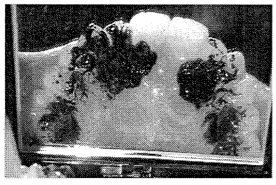
\includegraphics{../images/staticpalatography_fricative.png}
\end{figure}

~\\
INSTRUCTOR NOTES: no


\vfill
Excellent (3) ~~~ Good (2.2) ~~~ Fair (1.7) ~~~ Poor (0)
\newpage

{\large Question 4}\\

Source: Quiz 4, Question 1\\

L$_X$ (Language X) has three vowels, [i], [a], and [u]. It has bi-syllabic roots like Kikuyu. It does not allow non-identical high vowels to co-occur. Of the following nine logically possible vocalic sequences, which ones should be unattested in L$_X$? Explain why.\\

\begin{itemize} \item {[i...i]} \item {[i...a]} \item {[i...u]} \item {[a...i]} \item {[a...a]} \item {[a...u]} \item {[u...i]} \item {[u...a]} \item {[u...u]} \end{itemize}


~\\
INSTRUCTOR NOTES: [i...u], [u...i]


\vfill
Excellent (3) ~~~ Good (2.2) ~~~ Fair (1.7) ~~~ Poor (0)
\newpage

{\large Question 5}\\

Source: \\

What is the basic analysis of oral and nasal vowels in this dataset, and what are the key pieces of evidence?\\

\begin{figure}[H]
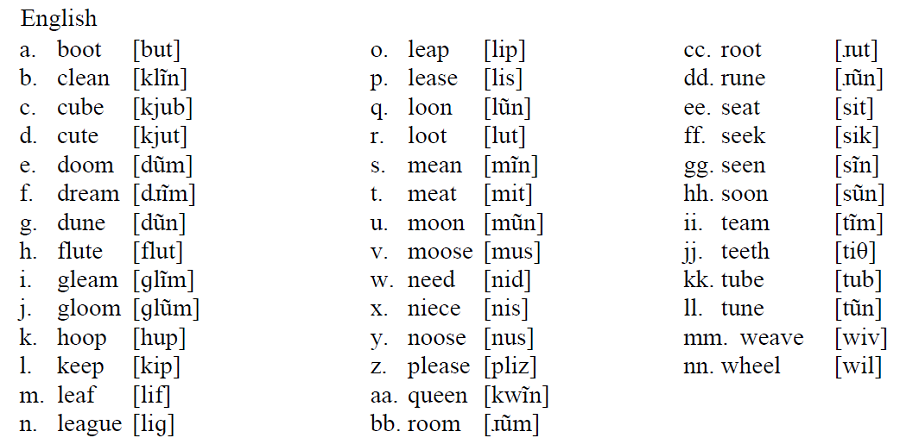
\includegraphics{../images/english12.png}
\end{figure}

~\\
INSTRUCTOR NOTES: The pairs of sounds [i] and [ĩ], and [u] and [ũ], are each allophonic and therefore allophones of the same phoneme in English (though the two pairs represent two contrastive phonemes in English). The sounds [i] and [ĩ] are in complementary distribution in English, with [ĩ] occurring before the sounds [m] and [n], (e.g., [ɡlĩm] ‘gleam’ and [klĩn] ‘clean’) and [i] occurring elsewhere (e.g., [lip] ‘leap’). Similarly, the sounds [u] and [ũ] are also in complementary distribution, with exactly the same conditioning environments: [ũ] occurs before [m] and [n] (e.g., [dũm] ‘doom’ and [dũn] ‘dune’), and [u] occurs elsewhere (e.g. [but] ‘boot’). Thus, within each pair, we treat the vowels as allophonic. 


\vfill
Excellent (3) ~~~ Good (2.2) ~~~ Fair (1.7) ~~~ Poor (0)
\newpage

\begin{center}
\textbf{{\color{red}{\HUGE END OF EXAM}}}\\

\end{center}
\newpage

\begin{center}
\textbf{{\color{blue}{\HUGE START OF EXAM\\}}}

\textbf{{\color{blue}{\HUGE Student ID: 84480\\}}}

\textbf{{\color{blue}{\HUGE \\}}}

\end{center}
\newpage

{\large Question 1}\\

Source: Quiz 2, Question 6\\

In the pronunciation of this word, which sounds are obstruents and which are sonorants?\\

<sonorant>


~\\
INSTRUCTOR NOTES: [sɔnoɹənt] -- sonorants: [ɔnoɹən] and obstruents: [st]


\vfill
Excellent (3) ~~~ Good (2.2) ~~~ Fair (1.7) ~~~ Poor (0)
\newpage

{\large Question 2}\\

Source: Week 2 Handout, Part II, Question 2\\

Explain why people might legitimately disagree about how many sounds this particular word contains.\\

<how>


~\\
INSTRUCTOR NOTES: 


\vfill
Excellent (3) ~~~ Good (2.2) ~~~ Fair (1.7) ~~~ Poor (0)
\newpage

{\large Question 3}\\

Source: Quiz 3, Question 12\\

Explain how you figure out which feature is involved in the process of umlaut shown below.\\

\begin{figure}[H]
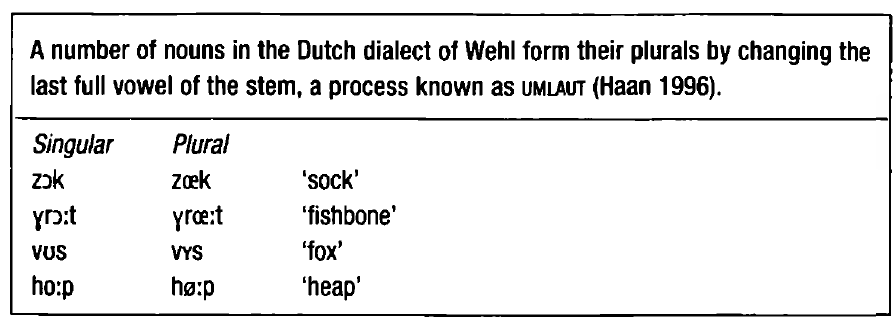
\includegraphics{../images/dutch.png}
\end{figure}

~\\
INSTRUCTOR NOTES: we look to see which vowels are affected, and compare them to see which feature is DIFFERENT (not e.g. what features they share); so since the vowels in the singular and plural are identical except that the singular forms are back and the plural are front, it's the feature [back] that is relevant / changing / involved (not e.g. the feature [round] just because all of the vowels are round)


\vfill
Excellent (3) ~~~ Good (2.2) ~~~ Fair (1.7) ~~~ Poor (0)
\newpage

{\large Question 4}\\

Source: Week 5 Handout, Question 5\\

How would you look for co-occurrence restrictions between [s] and the vowels that come after it in this dataset?\\

\begin{figure}[H]
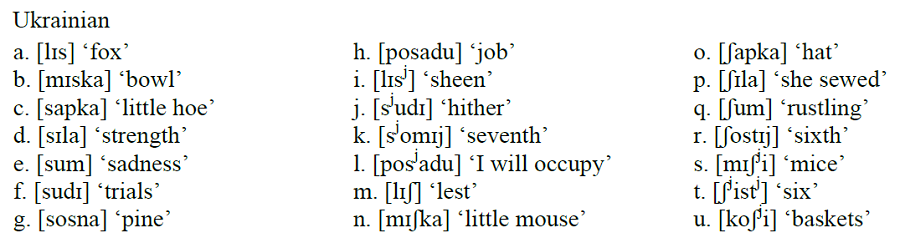
\includegraphics{../images/ukrainian.png}
\end{figure}

~\\
INSTRUCTOR NOTES: 


\vfill
Excellent (3) ~~~ Good (2.2) ~~~ Fair (1.7) ~~~ Poor (0)
\newpage

{\large Question 5}\\

Source: Week 6 Handout, Question 11\\

What do the two signs below tell you about the phonological status of \underline{handshape} in ASL, and why?\\

\begin{figure}[H]
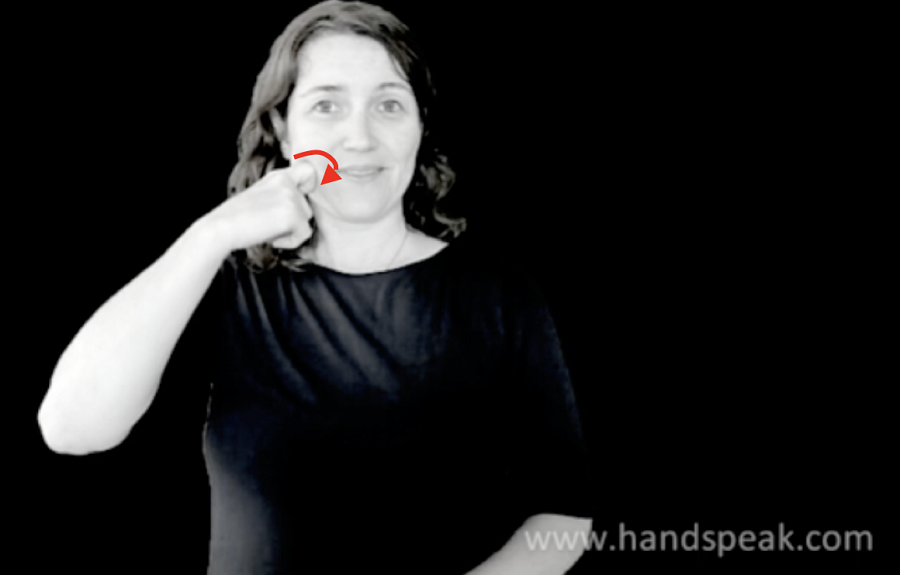
\includegraphics{../images/asl_apple.png}
\caption{APPLE}
\end{figure}
\begin{figure}[H]
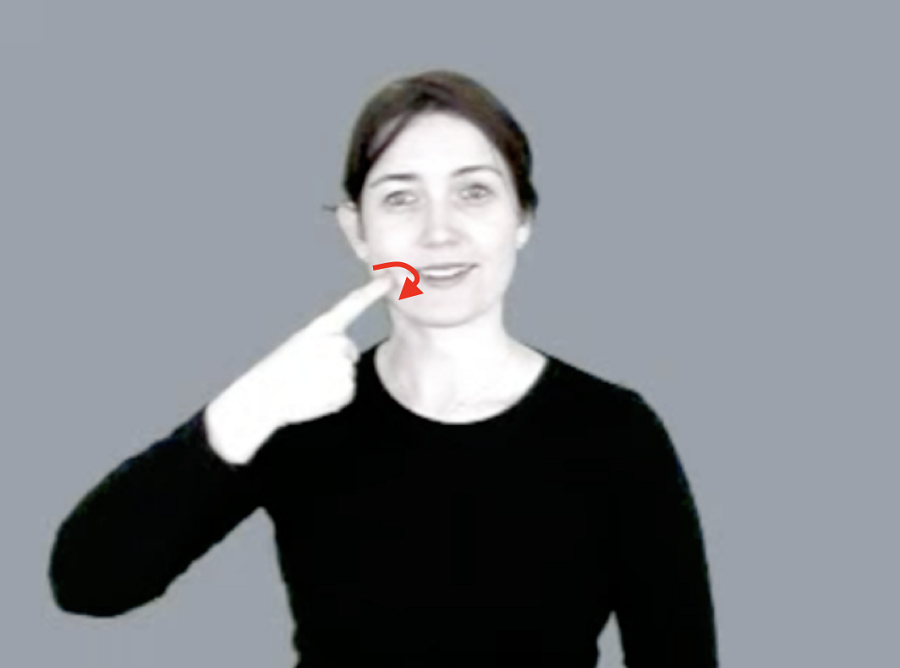
\includegraphics{../images/asl_candy.png}
\caption{CANDY}
\end{figure}

~\\
INSTRUCTOR NOTES: shows contrast because movement and location are same


\vfill
Excellent (3) ~~~ Good (2.2) ~~~ Fair (1.7) ~~~ Poor (0)
\newpage

\begin{center}
\textbf{{\color{red}{\HUGE END OF EXAM}}}\\

\end{center}
\newpage

\begin{center}
\textbf{{\color{blue}{\HUGE START OF EXAM\\}}}

\textbf{{\color{blue}{\HUGE Student ID: 85868\\}}}

\textbf{{\color{blue}{\HUGE \\}}}

\end{center}
\newpage

{\large Question 1}\\

Source: Week 5 Handout, Question 3\\

What evidence is there that there is a pattern in these data, assuming that these are the only CV and VC sequences that occur in some language?\\

{[sa]}, {[ʃi]}, {[za]}, {[ʒi]}, {[as]}, {[iʃ]}, {[az]}, {[iʒ]}


~\\
INSTRUCTOR NOTES: (the palatal sounds occur with the high vowel, while the alveolar sounds occur with the low vowel)


\vfill
Excellent (3) ~~~ Good (2.2) ~~~ Fair (1.7) ~~~ Poor (0)
\newpage

{\large Question 2}\\

Source: Week 2 Handout, Part II, Question 11\\

How would this word be transcribed?\\ Kathleen will likely ask a follow-up question about why you used a particular symbol.\\

<little>


~\\
INSTRUCTOR NOTES: [lɪɾl̩]


\vfill
Excellent (3) ~~~ Good (2.2) ~~~ Fair (1.7) ~~~ Poor (0)
\newpage

{\large Question 3}\\

Source: Quiz 3, Question 6\\

Explain why this is an incorrect statement.\\

Nasal consonants are {[+continuant]}, because you can continue to make the sound for a long period of time (until you run out of breath).


~\\
INSTRUCTOR NOTES: nasals are [-cont], because air cannot escape through the mouth


\vfill
Excellent (3) ~~~ Good (2.2) ~~~ Fair (1.7) ~~~ Poor (0)
\newpage

{\large Question 4}\\

Source: Week 3 Handout, Question 7\\

Is the symbol given a reasonable way to transcribe any of the sounds described below? If so, which one? If not, why not?\\

{[n]}

\begin{itemize} \item voiceless palatal affricate \item voiced velar nasal \item voiceless glottal fricative \item voiced labiodental fricative \item voiced interdental fricative \item voiced palatal fricative \end{itemize}


~\\
INSTRUCTOR NOTES: no (voiced alveolar nasal)


\vfill
Excellent (3) ~~~ Good (2.2) ~~~ Fair (1.7) ~~~ Poor (0)
\newpage

{\large Question 5}\\

Source: \\

What is the basic analysis of vowel length in this dataset, and what are the key pieces of evidence?\\

\begin{figure}[H]
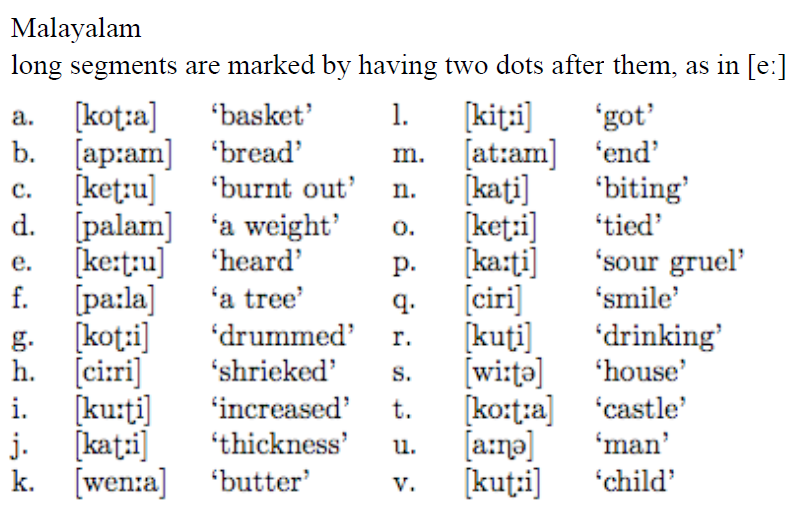
\includegraphics{../images/malayalam.png}
\end{figure}

~\\
INSTRUCTOR NOTES: Short and long vowels appear to be contrastive (phonemic) in Malayalam, as evidenced by minimal pairs that differ only in terms of their vowel length, such as [koʈːa] ‘basket’ vs. [koːʈːa] ‘castle’ or [keʈːu] ‘burnt out’ vs. [keːʈːu] ‘heard.’


\vfill
Excellent (3) ~~~ Good (2.2) ~~~ Fair (1.7) ~~~ Poor (0)
\newpage

\begin{center}
\textbf{{\color{red}{\HUGE END OF EXAM}}}\\

\end{center}
\newpage

\begin{center}
\textbf{{\color{blue}{\HUGE START OF EXAM\\}}}

\textbf{{\color{blue}{\HUGE Student ID: 99999\\}}}

\textbf{{\color{blue}{\HUGE \\}}}

\end{center}
\newpage

{\large Question 1}\\

Source: Week 5 Handout, Question 5\\

How would you look for co-occurrence restrictions between [s] and the vowels that come after it in this dataset?\\

\begin{figure}[H]
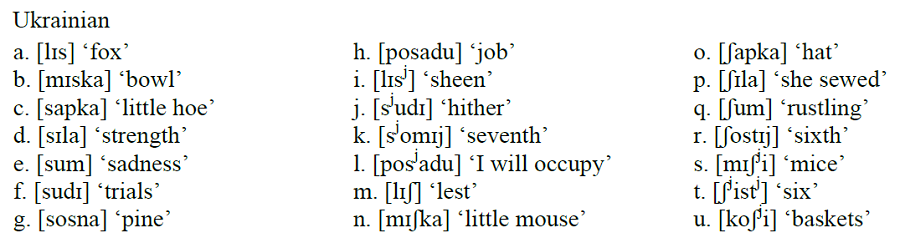
\includegraphics{../images/ukrainian.png}
\end{figure}

~\\
INSTRUCTOR NOTES: 


\vfill
Excellent (3) ~~~ Good (2.2) ~~~ Fair (1.7) ~~~ Poor (0)
\newpage

{\large Question 2}\\

Source: Week 4 Discussion\\

Explain what the given feature’s value is for this class of sounds, and why.\\

{[strident]}

glides


~\\
INSTRUCTOR NOTES: 0, because [strident] applies only to obstruents, and glides are sonorants


\vfill
Excellent (3) ~~~ Good (2.2) ~~~ Fair (1.7) ~~~ Poor (0)
\newpage

{\large Question 3}\\

Source: Week 2 Handout, Part II, Question 2\\

Explain why people might legitimately disagree about how many sounds this particular word contains.\\

<how>


~\\
INSTRUCTOR NOTES: 


\vfill
Excellent (3) ~~~ Good (2.2) ~~~ Fair (1.7) ~~~ Poor (0)
\newpage

{\large Question 4}\\

Source: Week 2 Discussion\\

Explain why it's possible to say that signed languages have articulatory phonetics.\\


~\\
INSTRUCTOR NOTES: 


\vfill
Excellent (3) ~~~ Good (2.2) ~~~ Fair (1.7) ~~~ Poor (0)
\newpage

{\large Question 5}\\

Source: \\

What is the basic analysis of oral and nasal vowels in this dataset, and what are the key pieces of evidence?\\

\begin{figure}[H]
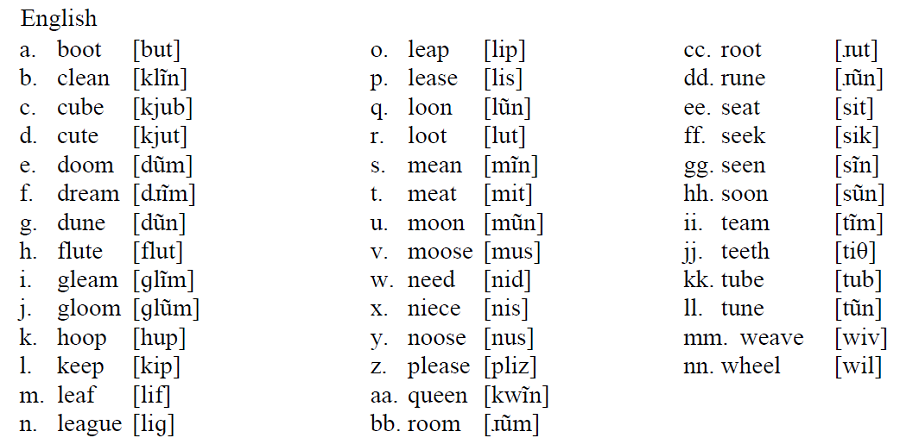
\includegraphics{../images/english12.png}
\end{figure}

~\\
INSTRUCTOR NOTES: The pairs of sounds [i] and [ĩ], and [u] and [ũ], are each allophonic and therefore allophones of the same phoneme in English (though the two pairs represent two contrastive phonemes in English). The sounds [i] and [ĩ] are in complementary distribution in English, with [ĩ] occurring before the sounds [m] and [n], (e.g., [ɡlĩm] ‘gleam’ and [klĩn] ‘clean’) and [i] occurring elsewhere (e.g., [lip] ‘leap’). Similarly, the sounds [u] and [ũ] are also in complementary distribution, with exactly the same conditioning environments: [ũ] occurs before [m] and [n] (e.g., [dũm] ‘doom’ and [dũn] ‘dune’), and [u] occurs elsewhere (e.g. [but] ‘boot’). Thus, within each pair, we treat the vowels as allophonic. 


\vfill
Excellent (3) ~~~ Good (2.2) ~~~ Fair (1.7) ~~~ Poor (0)
\newpage

\begin{center}
\textbf{{\color{red}{\HUGE END OF EXAM}}}\\

\end{center}
\newpage

\end{document}

